%!TEX root = ../document.tex
\chapter{Broken Authentication and Session Management}
\label{BrokenAuthenticationAndSessionManagement}
\subsubsection*{Von: Juliane Hauser, Kristina Linz}
\section{Erklärung}
Diese Sicherheitslücke befindet sich im OWASP Top 10 Risk Rating 2017 auf dem 2. Platz (OWASP A2). 
Auf vielen Web-Applikationen wird eine Benutzerauthentifizierung mit Benutzername und Passwort benötigt, um deren Dienste zu nutzen. Beispiele hierfür sind Online-Shops, Social-Media-Plattformen und Online-Banking. 
\\
Für die Interaktion zwischen dem angemeldeten Benutzer und der Web-Applikation ist das Session-Management nötig, wobei die gesammelten Session-Informationen in Cookies unter der eindeutigen Session-ID der Benutzer-Session abgespeichert werden. Cookies werden vom Browser verwendet, um client-seitig Informationen abzuspeichern.
\\
Der technische Hintergrund ist die Zustandslosigkeit des HTTP-Protokolls. Das HTTP-Protokoll wird für die Kommunikation zwischen dem Client und dem Web-Server eingesetzt. Die Zustandslosigkeit führt dazu, dass der Web-Server Seitenaufrufe unabhängig voneinander interpretiert und keinen Zusammenhang herstellen kann. Mit Hilfe des Session-Managements werden die Seitenaufrufe eines Benutzers in einer Session einander zugeordnet. Die Session-ID ist eine lange und zufällige Zeichenkette, wobei sichergestellt werden muss, dass dieser Identifier eindeutig und nicht leicht zu erraten ist.
\\
Als mögliche Konsequenz von Fehlern in der Authentifizierung und dem Session-Management folgt die Kompromittierung oder Übernahme von Benutzerkonten.

\subsection{Fehler in der Authentifizierung}
Wenn die Passwort-Policy für die Registrierung nicht ausreichend streng ist, verleitet dies Benutzer dazu schwache Passwörter zu verwenden. Dadurch wird ein Brute-Force-Angriff möglich, wobei durch systematisches Probieren aller möglichen Kombinationen die Benutzernamen und dazugehörigen Passwörter fremder Benutzer erraten werden können.\\\\
Eine weitere Fehlerquelle ist die Verschlüsselung von Benutzername und Passwort. Wenn diese Daten im Klartext über das HTTP-Protokoll versendet werden, ist es einem Angreifer möglich die Kommunikation abzuhören. Wenn beim Abspeichern der Benutzerdaten auf Hash-Verfahren bzw. Verschlüsselung verzichtet wird, sind diese Daten ungeschützt vor anderen Sicherheitslücken wie beispielsweise SQL-Injections.\\
Teilweise gibt der Web-Server aussagekräftige Informationen über bereits bestehende Benutzerkonten Preis, sodass ein fremdes Benutzerkonto übernommen werden kann. Bei der Konto-Erstellung oder "Passwort-Zurücksetzen"-Funktion kann ggf. ein bestehender Benutzername ermittelt werden. Der Benutzername stellt bereits die erste Hälfte der Lösung des Benutzername-Passwort-Rätsels dar.

\subsection{Fehler im Session-Management}
Ist die Wahl der Session-ID nicht ausreichend zufällig gestaltet, besteht die Möglichkeit, dass eine gültige Session-ID erraten wird. Wenn zudem die Session-ID als Parameter in der URL übergeben wird, ist es einem Dritten möglich die Session zu übernehmen. Dieser Dritte kann dadurch alle Funktionen der Web-Applikation mit den Berechtigungen des angemeldeten Benutzers verwenden. Wird die URL unverschlüsselt übertragen, kann ein Angreifer ebenfalls eine fremde Session-ID ermitteln und die Session eines angemeldeten Benutzers übernehmen. Das HTTPS-Protokoll bietet eine Verschlüsselung für diese Problematik.\\
Wenn Session-IDs nach dem Abmelden eines Benutzers nicht auf ungültig gesetzt werden, können diese zur Wiederherstellung der Anwender-Session missbraucht werden. Ebenso werden Session-IDs zu vorhersehbar, wenn diese sich nicht mit erneuter Anmeldung ändern.\\
Wenn das HttpOnly-Attribut nicht gesetzt wird, ist das Auslesen des Session-Cookies über Skriptsprachen möglich. Im Rahmen eines XSS-Angriffs kann die Session-ID eines anderen Benutzers ermittelt werden. 

\subsection{Gegenmaßnahmen}
Die Authentifizierungsfunktion ist so zu gestalten, dass nach wiederholter Fehleingabe der Anmeldedaten das Benutzerkonto oder die Aufrufer-IP temporär gesperrt werden.\\
Außerdem sollte weder bei der Registrierung noch bei der "Passwort-Vergessen"-Funktion eine aussagekräftige Rückmeldung über bereits existierende Benutzernamen gegeben werden. Wenn dies aus Gründen der Benutzerfreundlichkeit nicht möglich ist, sind zumindest automatisierte Abfragen zu unterbinden.\\\\
Die Übermittlung der Anmeldedaten sollte ausschließlich verschlüsselt mit TLS und die Speicherung der Passwörter in gehashter Form mit geeigneten kryptographischen Funktionen gestaltet werden.\\
Session-IDs sind ausreichend zufällig zu wählen, nicht unverschlüsselt zu übertragen und bei einer Abmeldung serverseitig zu beenden. Zum Erzwingen der Verschlüsselten Übertragung der Session-ID wird das Secure-Attribut des Session-Cookies aktiviert. Außerdem ist es ratsam das HttpOnly-Attribut zu setzen, um ein Auslesen des Cookies mittels JavaScript zu verhindern.\\
Um Session-Übernahmen zu vermeiden, ist es darüber hinaus möglich, die Session des Anwenders mit spezifischen Nutzermerkmalen, beispielsweise dem entsprechenden User-Agent oder der IP-Adresse zu verknüpfen.\\
Neben diesen Standardmaßnahmen sind auch die von der OWASP formulierten Anforderungen an Authentifizierung und Session-Management umzusetzen. Diese sind in den OWASP Application Security Verification Standards beschrieben.\\
\\
Quelle:\\ https://www.datenschutz-notizen.de/owasp-top-ten-a2-fehler-in-authentifizierung-und-session-management-2713238/

\section{Übungen}
\subsection{Registrierung}
Das Lernziel der ersten Übung zum Thema Registrierung ist es, dem Anwender gängige Passwortregeln aufzuzeigen. Inhalt der Übung ist es, sich erfolgreich zu registrieren unter Einhaltung gängiger Passwortregeln. Die Startseite der Übung ist Abbildung \ref{fig:Aufgabe 1 Registrierung} zu entnehmen.\\


\begin{figure}[]
	
	\centering
	
	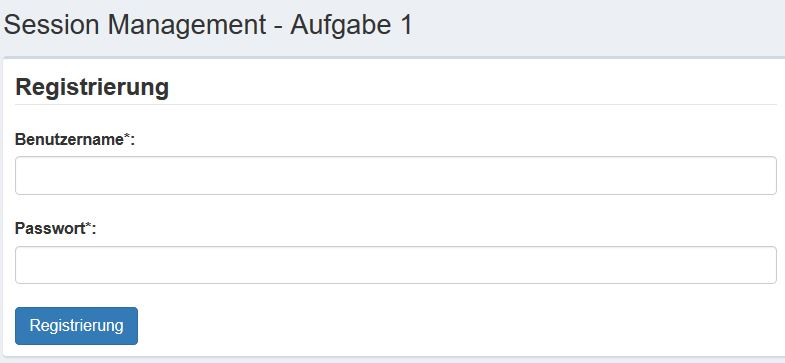
\includegraphics[width=1.0\linewidth]{images/BrokenAuthenticationAndSessionManagement/Registrierung_Start}
	
	\caption[Aufgabe 1: Registrierung nach gängigen Passwortregeln.]{Registrierung nach gängigen Passwortregeln.}
	
	\label{fig:Aufgabe 1 Registrierung}
	
\end{figure}
\noindent In dieser Übung werden zwei Hinweise zur Verfügung gestellt. Der erste Hinweis ist, dass das gewählte Passwort den allgemein üblichen Regeln zu entsprechen hat, damit die Registrierung erfolgreich durchgeführt werden kann. Im zweiten Hinweis werden die verwendeten Passwortregeln aufgelistet: Länge von mind. 8 Zeichen, mind. ein Großbuchstabe, mind. ein Kleinbuchstabe und eine Zahl. \\
Nach erfolgreicher Registrierung wird der Benutzer auf die in Abbildung \ref{fig:Aufgabe 1 Abschluss} dargestellte Seite weitergeleitet und hat die Aufgabe erfolgreich gelöst.\\
\begin{figure}[H]
	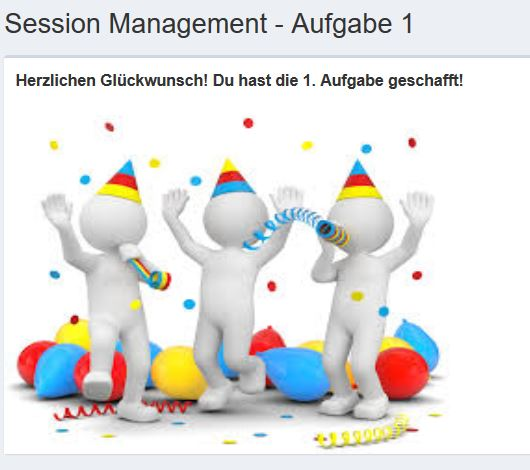
\includegraphics[width=1.0\linewidth]{images/BrokenAuthenticationAndSessionManagement/Registrierung_Ende}
	\caption[Landing-Page nach erfolgreicher Registrierung.]{Landing-Page nach erfolgreicher Registrierung.}
	\label{fig:Aufgabe 1 Abschluss}
\end{figure}
\subsection{Login}
Das Ziel der zweiten Übung liegt darin aufzuzeigen, wie leicht Passwörter zu erraten sind, wenn die gängigen Passwortregeln nicht einzuhalten sind. Es gibt sehr beliebte und einfache Benutzername- und Passwort-Kombinationen, die in dieser Übung ausgenutzt werden.\\ 
Die Aufgabenstellung ist deshalb so gewählt, dass sich der Benutzer mit einem fremden, unbekannten Benutzerkonto anmelden soll. Dabei sind Benutzername und Passwort zu erraten. \\
\begin{figure}[H]
	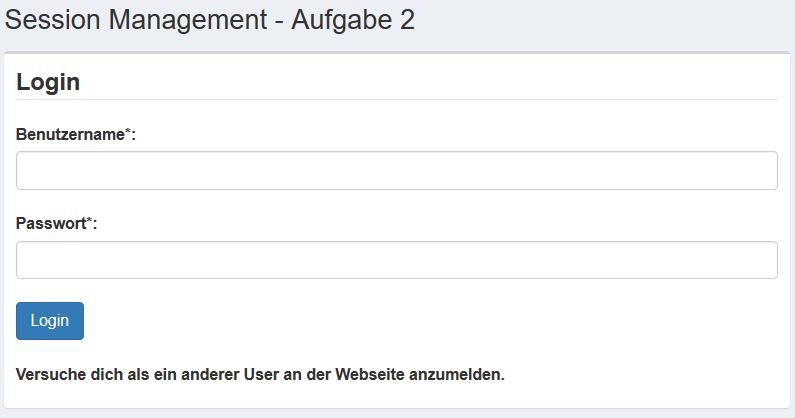
\includegraphics[width=1.0\linewidth]{images/BrokenAuthenticationAndSessionManagement/Login_Start}
	\caption[Aufgabe 2: Login.]{Aufgabe 2: Login.}
	\label{fig:Aufgabe 2 Login}
\end{figure}
\noindent Bei Bedarf werden zwei Hinweise gegeben. Der erste Hinweis ist, dass es sich hier um sehr einfache, beliebte Benutzernamen und Passwörter handelt. Wenn dieser Tipp nicht ausreicht, wird im zweiten Hinweis ein existierendes Passwort ('admin') vorgegeben. Zu diesem Benutzername würde das Passwort 'admin' passen. Es gibt jedoch auch andere Kombinationen: z.B. Benutzername 'benutzer' und als Passwort 'passwort1' oder 'fußballfan' und 'schalke04'.\\
Einige dieser beliebten Benutzernamen und Passwörter sind in der Datenbank der Webseite hinterlegt.\\\\\\\\\\\\
Bei erfolgreicher Anmeldung mit einem fremden Benutzerkonto, gelangt der Benutzer zur letzten Seite dieser Übung:
\begin{figure}[H]
	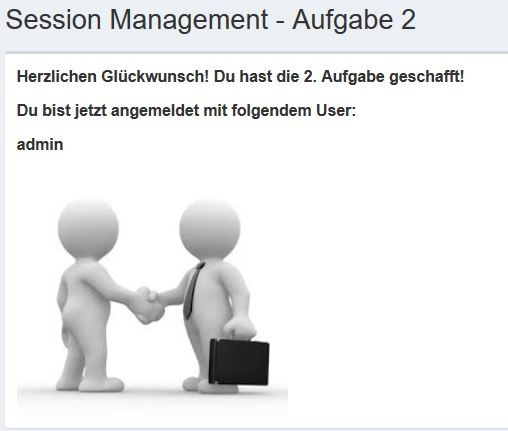
\includegraphics[width=1.0\linewidth]{images/BrokenAuthenticationAndSessionManagement/Login_Ende}
	\caption[Landing-Page nach erfolgreichem Login.]{Landing-Page nach erfolgreichem Login.}
	\label{fig:Aufgabe 2 Abschluss}
\end{figure} 
\noindent Durch das Erraten von Benutzername und Passwort, ist es möglich die Funktionen der Webapplikation mit den Berechtigungen des fremden Benutzerkontos zu nutzen. In unserer Übung wird das jedoch nicht mehr abgefragt.
\subsection{Logout}
Das Lernziel der dritten Übung ist die Erkenntnis, dass nach einem Logout die Session zwingend beendet werden muss und die dazugehörigen Daten nicht mehr verfügbar sein dürfen.\\\\\\
Die Aufgabenstellung liegt darin, nach dem Logout ohne erneute Anmeldung zurück zu der Webseite als angemeldeter Benutzer zu gelangen.\\ 
\begin{figure}[H]
	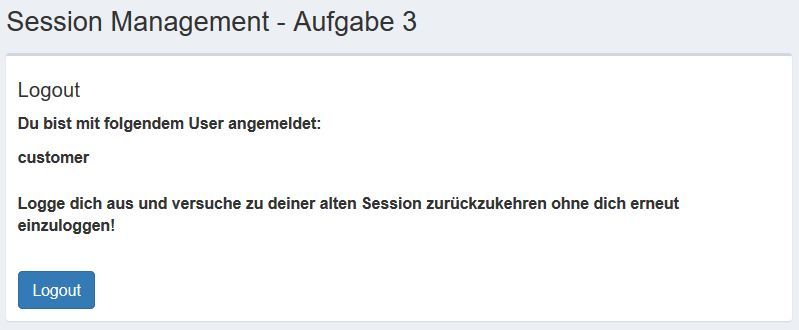
\includegraphics[width=1.0\linewidth]{images/BrokenAuthenticationAndSessionManagement/Logout_Start}
	\caption[Aufgabe 3: Logout.]{Aufgabe 3: Logout.}
	\label{fig:Aufgabe 3 Logout}
\end{figure}



\noindent Durch das Klicken auf den Logout-Button erfolgt eine Weiterleitung zur Logout-Seite. Diese ist in Abbildung \ref{fig:Aufgabe 3 Abschluss} abgebildet.\\\\
\begin{figure}
	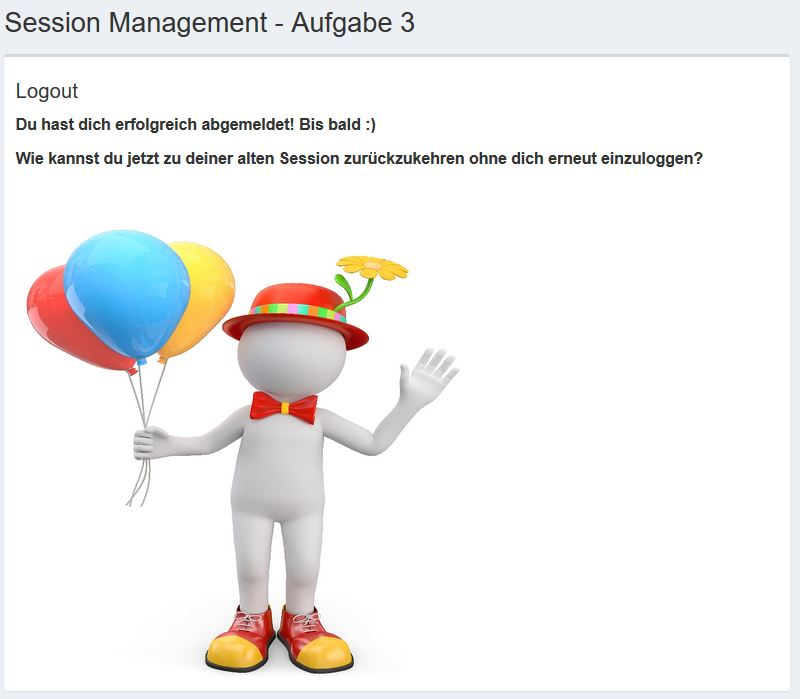
\includegraphics[width=1.0\linewidth]{images/BrokenAuthenticationAndSessionManagement/Logout_Mitte}
	\caption[Logout-Seite.]{Logout-Seite.}
	\label{fig:Aufgabe 3 Abschluss}
\end{figure}

\noindent Hier wird der Hinweis, dass der Browser eine 'zurück'-Funktion bietet, bei Bedarf zur Verfügung gestellt.\\
Wird die Funktion des Browsers ausgenutzt, gelangt der Benutzer wieder zur Startseite der Übung und erscheint als angemeldeter Benutzer. Somit ist die Übung erfolgreich absolviert.\\\\\\\\\\\\\\\\\\\\\\\\\\
\subsection{URL-Manipulation}
Mithilfe der letzten Übung wird gezeigt, dass Session-Attribute und die Session-ID nicht sichtbar übertragen werden sollten, wie z.B. in der URL. Zudem darf die Session-ID nicht spechend wie beispielsweise der Benutzername gewählt werden. Es ist besser, wenn die Session-ID einer willkürlichen Zeichenfolge entspricht.\\
Die Aufgabenstellung besteht darin, das Benutzerkonto des Admins zu übernehmen. Aktuell ist der Benutzer 'customer' angemeldet.\\
\begin{figure}[H]
	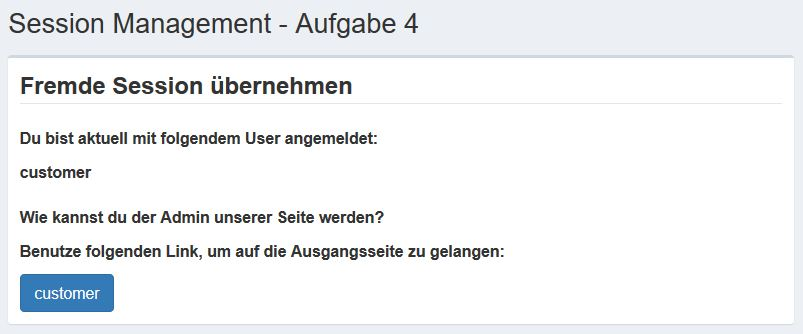
\includegraphics[width=1.0\linewidth]{images/BrokenAuthenticationAndSessionManagement/URL_Start}
	\caption[Aufgabe 4: URL-Manipulation.]{Aufgabe 4: URL-Manipulation.}
	\label{fig:Aufgabe 4 URL-Manipulation}
\end{figure}
\noindent Durch Betätigung des Buttons 'customer', gelangt der Benutzer zur Ausgangsseite:
\begin{figure}[H]
	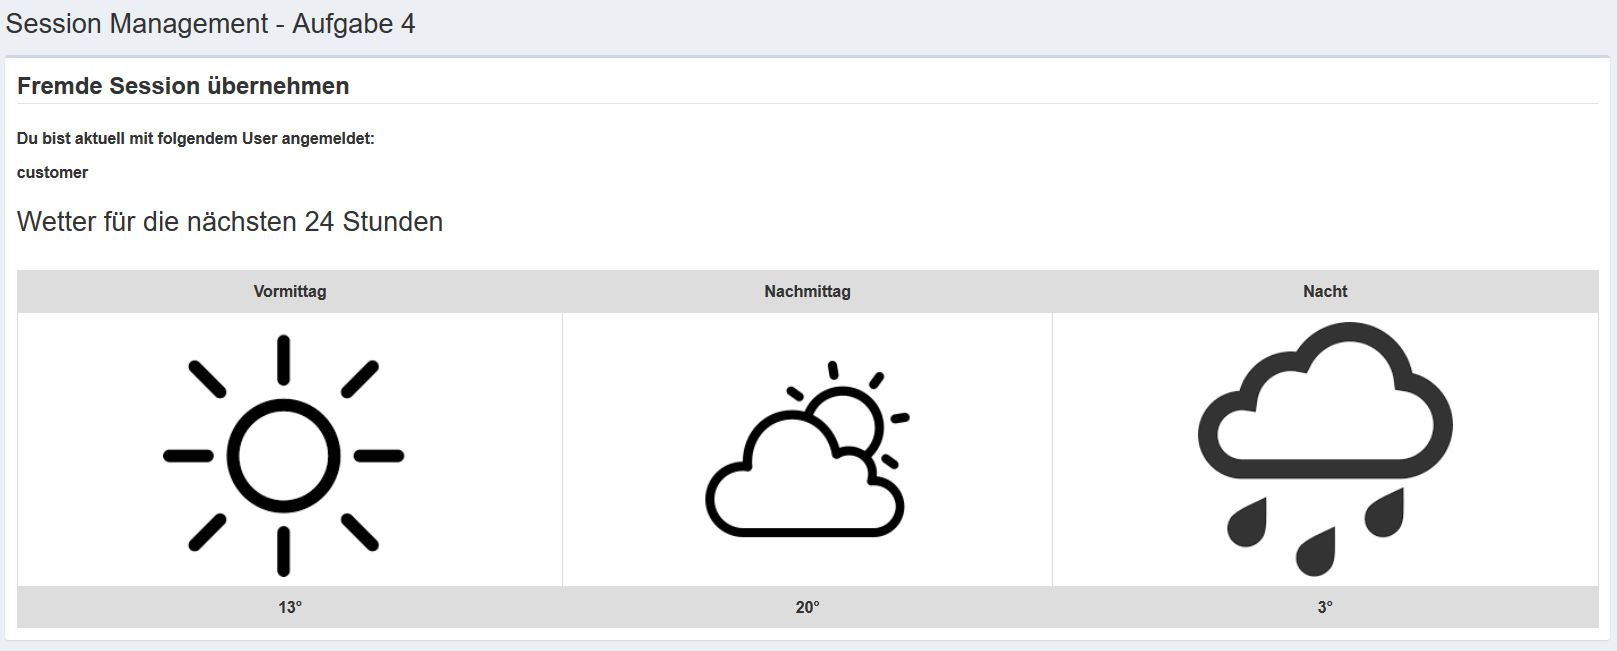
\includegraphics[width=0.95\linewidth]{images/BrokenAuthenticationAndSessionManagement/URL_customer}
	\caption[Aufgabe 4: Ausgangsseite des Customers.]{Aufgabe 4: Ausgangsseite des Customers.}
	\label{fig:Aufgabe 4 Ausgangsseite des Customers}
\end{figure}
\noindent Auf der Ausgangsseite werden zwei Hinweise angeboten. Der erste Tipp, weißt auf die Unterschiede des GET- und POST-Requests des HTTP-Protokolls hin. Der zweite Tipp lenkt die Aufmerksamkeit des Anwenders auf die Parameter der URL, die zu manipulieren sind.\\
Die Parameter in der URL entsprechen dem Lösungsweg, da hier der Username hinterlegt ist.
\begin{figure}[H]
	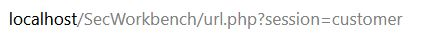
\includegraphics[width=1.0\linewidth]{images/BrokenAuthenticationAndSessionManagement/URL_customer_url}
	\caption[Aufgabe 4: URL der Ausgangsseite des Customers.]{Aufgabe 4: URL der Ausgangsseite des Customers.}
	\label{fig:Aufgabe 4 URL der Ausgangsseite des Customers}
\end{figure} 
\noindent Wird der Wert des Session-Parameters von 'customer' auf 'admin' geändert, gelang der Benutzer zur Session des Admins.
\begin{figure}[H]
	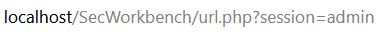
\includegraphics[width=1.0\linewidth]{images/BrokenAuthenticationAndSessionManagement/URL_admin_url}
	\caption[Aufgabe 4: URL der Ausgangsseite des Admins.]{Aufgabe 4: URL der Ausgangsseite des Admins.}
	\label{fig:Aufgabe 4 URL der Ausgangsseite des Admins}
\end{figure}
\noindent Für den Admin ist der Wetterbericht der nächsten drei Tage sichtbar, der Kunde sieht jedoch nur das Wetter der nächsten 24 Stunden. Wenn der Benutzer auf dieser Seite angelangt ist, hat er die letzte Übung erfolgreich abgeschlossen.
\begin{figure}[H]
	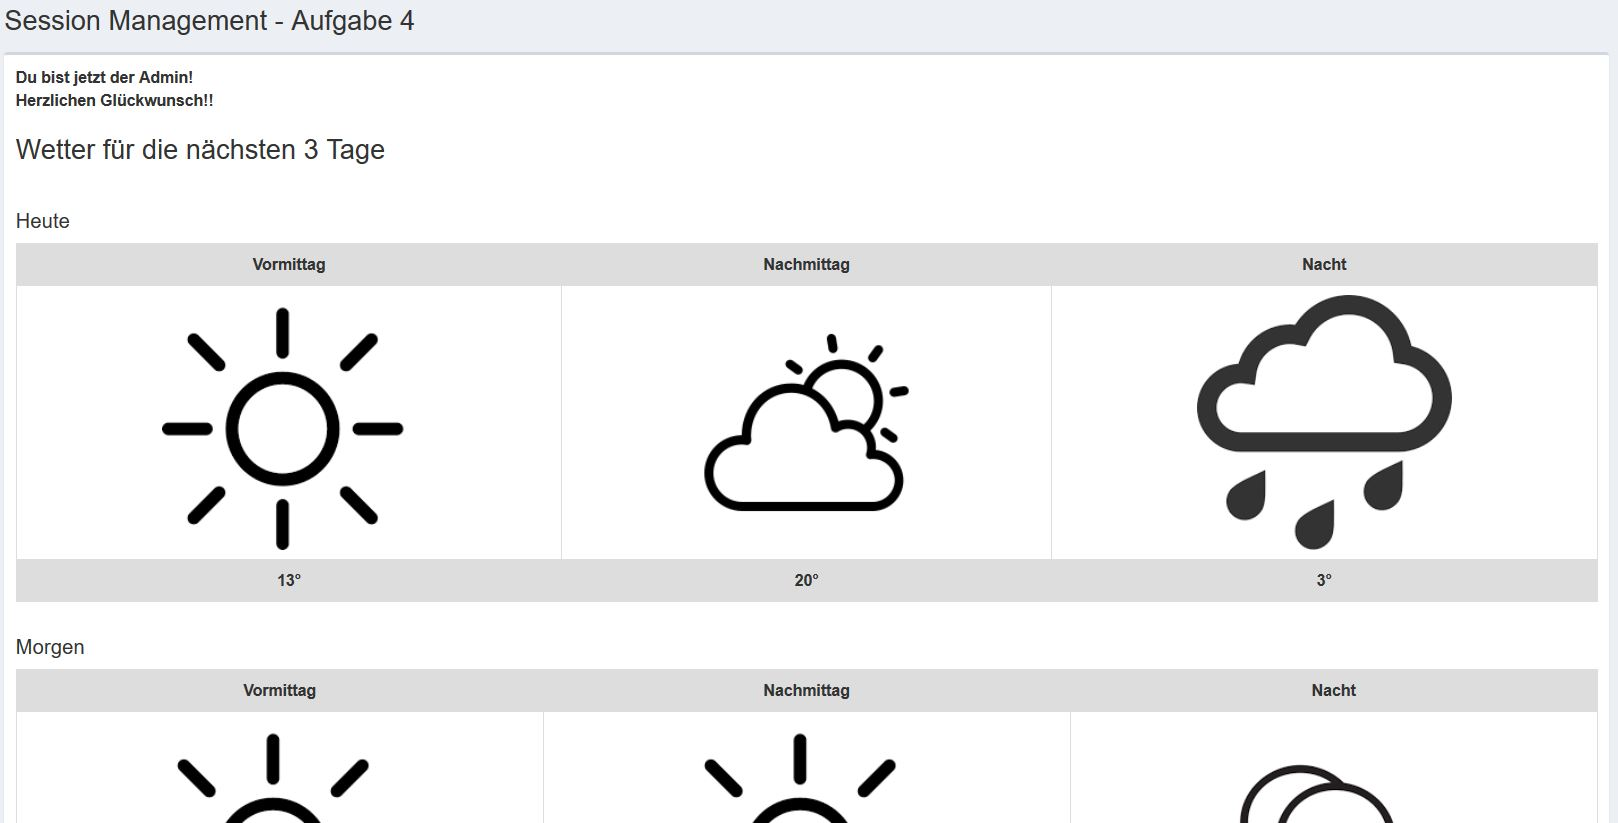
\includegraphics[width=1.0\linewidth]{images/BrokenAuthenticationAndSessionManagement/URL_admin}
	\caption[Aufgabe 4: Ausgangsseite des Admin.]{Aufgabe 4: Ausgangsseite des Admin.}
	\label{fig:Aufgabe 4 Ausgangsseite des Admin}
\end{figure}